\pagebreak\section{Interfacing a seven segment display}
\subsection{Experiment URL}
    Use this \href{https://www.tinkercad.com/things/cBjJt1Np6D3?sharecode=MGQeyKRCp2DAykyyOVjQAholeCilkMIFth6zI349h3c}{link} to get the \textbf{Tinkercad} simulation of this experiment.
    
\subsection{Objectives}


\subsection{Necessary Components}
We will need the following components −
\begin{itemize}
\item 1 x seven segment display (common cathode)
\item 1 x Arduino UNO R3
\item 1 x breadboard
\item 1 x 1k$\Omega$ resistors (1/4 W)
\item jumper wires
\end{itemize}
\subsection{Circuit Diagram}
        \begin{figure}[!h]
            \centering
            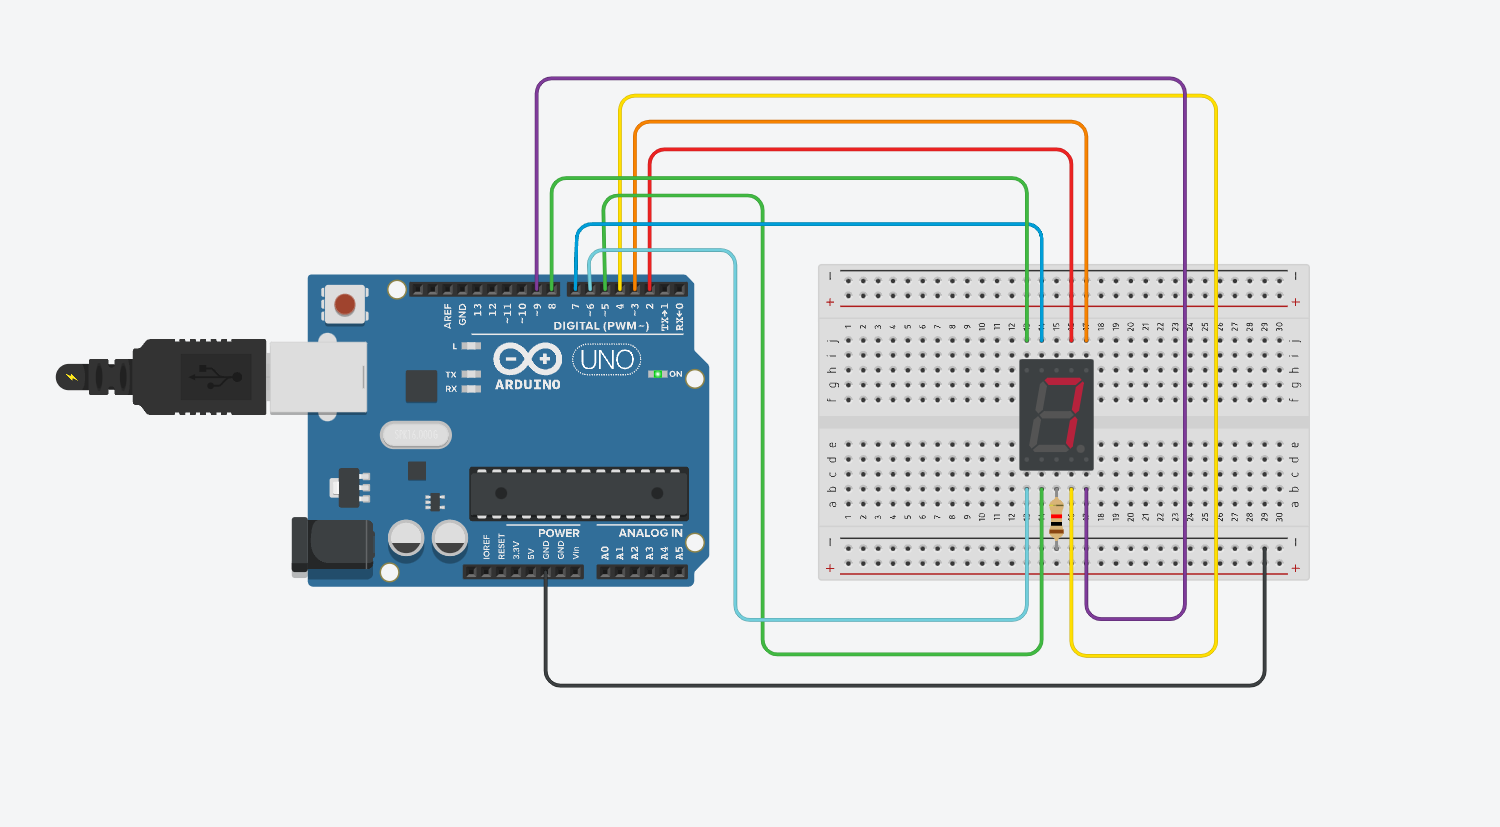
\includegraphics[width =0.85\textwidth]{images/seven_segment_display.png}
            \caption{Interfacing seven segment display with Arduino}
        \end{figure}

\pagebreak\subsection{Arduino Code}
    \begin{lstlisting}[style = Arduino]
/*Interfacing a seven segment display using Arduino*/
int i;
int pinA = 2;
int pinB = 3;
int pinC = 4;
int pinD = 5;
int pinE = 6;
int pinF = 7;
int pinG = 8;
int pinDP = 9;

void setup()
{
  for ( i = 2; i <= 9; i++){
  pinMode(i, OUTPUT);
}
}

void loop()
{
  // display 0
  digitalWrite(2, HIGH);
  digitalWrite(3, HIGH);
  digitalWrite(4, HIGH);
  digitalWrite(5, HIGH);
  digitalWrite(6, HIGH);
  digitalWrite(7, HIGH);
  digitalWrite(8, LOW);
  digitalWrite(9, LOW);
  delay(1000); // Wait for 1000 millisecond(s)
  // display 1
  digitalWrite(2, LOW);
  digitalWrite(3, HIGH);
  digitalWrite(4, HIGH);
  digitalWrite(5, LOW);
  digitalWrite(6, LOW);
  digitalWrite(7, LOW);
  digitalWrite(8, LOW);
  digitalWrite(9, LOW);
  delay(1000); // Wait for 1000 millisecond(s)
  // display 2
  digitalWrite(2, HIGH);
  digitalWrite(3, HIGH);
  digitalWrite(4, LOW);
  digitalWrite(5, HIGH);
  digitalWrite(6, HIGH);
  digitalWrite(7, LOW);
  digitalWrite(8, HIGH);
  digitalWrite(9, LOW);
  delay(1000); // Wait for 1000 millisecond(s)
  // display 3
  digitalWrite(2, HIGH);
  digitalWrite(3, HIGH);
  digitalWrite(4, HIGH);
  digitalWrite(5, HIGH);
  digitalWrite(6, LOW);
  digitalWrite(7, LOW);
  digitalWrite(8, HIGH);
  digitalWrite(9, LOW);
  delay(1000); // Wait for 1000 millisecond(s)
  // display 4
  digitalWrite(2, LOW);
  digitalWrite(3, HIGH);
  digitalWrite(4, HIGH);
  digitalWrite(5, LOW);
  digitalWrite(6, LOW);
  digitalWrite(7, HIGH);
  digitalWrite(8, HIGH);
  digitalWrite(9, LOW);
  delay(1000); // Wait for 1000 millisecond(s)
  // display 5
  digitalWrite(2, HIGH);
  digitalWrite(3, LOW);
  digitalWrite(4, HIGH);
  digitalWrite(5, HIGH);
  digitalWrite(6, LOW);
  digitalWrite(7, HIGH);
  digitalWrite(8, HIGH);
  digitalWrite(9, LOW);
  delay(1000); // Wait for 1000 millisecond(s)
  // display 6
  digitalWrite(2, HIGH);
  digitalWrite(3, LOW);
  digitalWrite(4, HIGH);
  digitalWrite(5, HIGH);
  digitalWrite(6, HIGH);
  digitalWrite(7, HIGH);
  digitalWrite(8, HIGH);
  digitalWrite(9, LOW);
  delay(1000); // Wait for 1000 millisecond(s)
  // display 7
  digitalWrite(2, HIGH);
  digitalWrite(3, HIGH);
  digitalWrite(4, HIGH);
  digitalWrite(5, LOW);
  digitalWrite(6, LOW);
  digitalWrite(7, LOW);
  digitalWrite(8, LOW);
  digitalWrite(9, LOW);
  delay(1000); // Wait for 1000 millisecond(s)
  // display 8
  digitalWrite(2, HIGH);
  digitalWrite(3, HIGH);
  digitalWrite(4, HIGH);
  digitalWrite(5, HIGH);
  digitalWrite(6, HIGH);
  digitalWrite(7, HIGH);
  digitalWrite(8, HIGH);
  digitalWrite(9, LOW);
  delay(1000); // Wait for 1000 millisecond(s)
  // display 9
  digitalWrite(2, HIGH);
  digitalWrite(3, HIGH);
  digitalWrite(4, HIGH);
  digitalWrite(5, LOW);
  digitalWrite(6, LOW);
  digitalWrite(7, HIGH);
  digitalWrite(8, HIGH);
  digitalWrite(9, LOW);
  delay(1000); // Wait for 1000 millisecond(s)
}

\end{lstlisting}